\documentclass[a4paper,12pt]{article}
\usepackage[pdftex]{graphicx}


\begin{document}


\begin{titlepage}

\begin{center}

{ \huge \bfseries Computer Network}\\[0.8cm]


\textsc{\LARGE Assignment -- 11}\\[1.5cm]

\begin{center}
 
\includegraphics{IITD.png}
 % iitd.jpg: 200x204 pixel, 96dpi, 5.29x5.40 cm, bb=0 0 150 153
\end{center}




{ \huge \bfseries Design Documentation}\\[0.4cm]
\textsc{\LARGE development of new module for NS2 (ARQ Support) }\\[1cm]
\textsc{\LARGE Harshit Kumar Gupta}\\[1.5cm]
\textsc{\LARGE Entry No. 2013EET2369}\\[0.5cm]

\end{center}

\end{titlepage}

\tableofcontents
\newpage
\section{Problem Statement}
\begin{itemize}
\item  We first design NS2 modules for limited persistence ARQ protocol (sample codes will be provided)
\item feedback channel is assumed to be error free
\item setup an experiment to show the impact of ARQ module on TCP throughput. Inser an error module with error prob. (make a Tcl simulation script)
\item make a folder in ~/ns-allinone-xxx/ns-xxx/<yourfolder>  and copy .c and .h files in this
\item 2 copy ns-lib.tcl and ns-link.tcl at their places
\item recompile complete ns2 and generate object file

\item make tcl simulation script to test your module
\item  make a error model and set its error rate from the argument passed while running the script
\item  use link-lossmodel  between n1 and n3
\item  use command link-arq defined in ns-lib.tcl with proper args
\item  make tcp connection between n1 and n3
\end{itemize}
\section{Assumptions :}
Assumptions made are:
\begin{itemize}
\item Only two link's are able to sand packet at a time.
\item The communication can be only between two distint link's.
\item The pkt drop according to the arq model or rate.
\item The communication between two nodes are only for 100.1s . 
\end{itemize}

\section{Specifications}
The following speciations are used in the assignment:
\begin{itemize}
\item  The link b/w nodes are dupliex.
\item  The arq model is work perfactly.
\item  The pkt is drop according to given condiction.
\end{itemize}





\section{Approach :}

\begin{enumerate}


\item  First write a network topology using tcl. Here the connections, source and sink are defined.
 \item Sample simulation can be seen using nam.
 \item then add the arq model in that script.
 \item On the terminal type ns [filename].tcl.
 \item It will generate a trace file which contains the details of packet movement through the network.
 \item Now write a awk script to parse the trace file can calculate throughput and interarrival time.
 \item Write another file using the awk script which contains columans for x and y-axis for the plot.
 \item On the terminal type awk -f [filename].awk [tracefile].
 \item Use this output file to generate plot. For this, type gnuplot. On the shell, type plot [filename].
 \item Analyse the results.
\end{enumerate}
\newpage
\section{Execution}
Topology as viewed on NAM : -
\begin{center}
 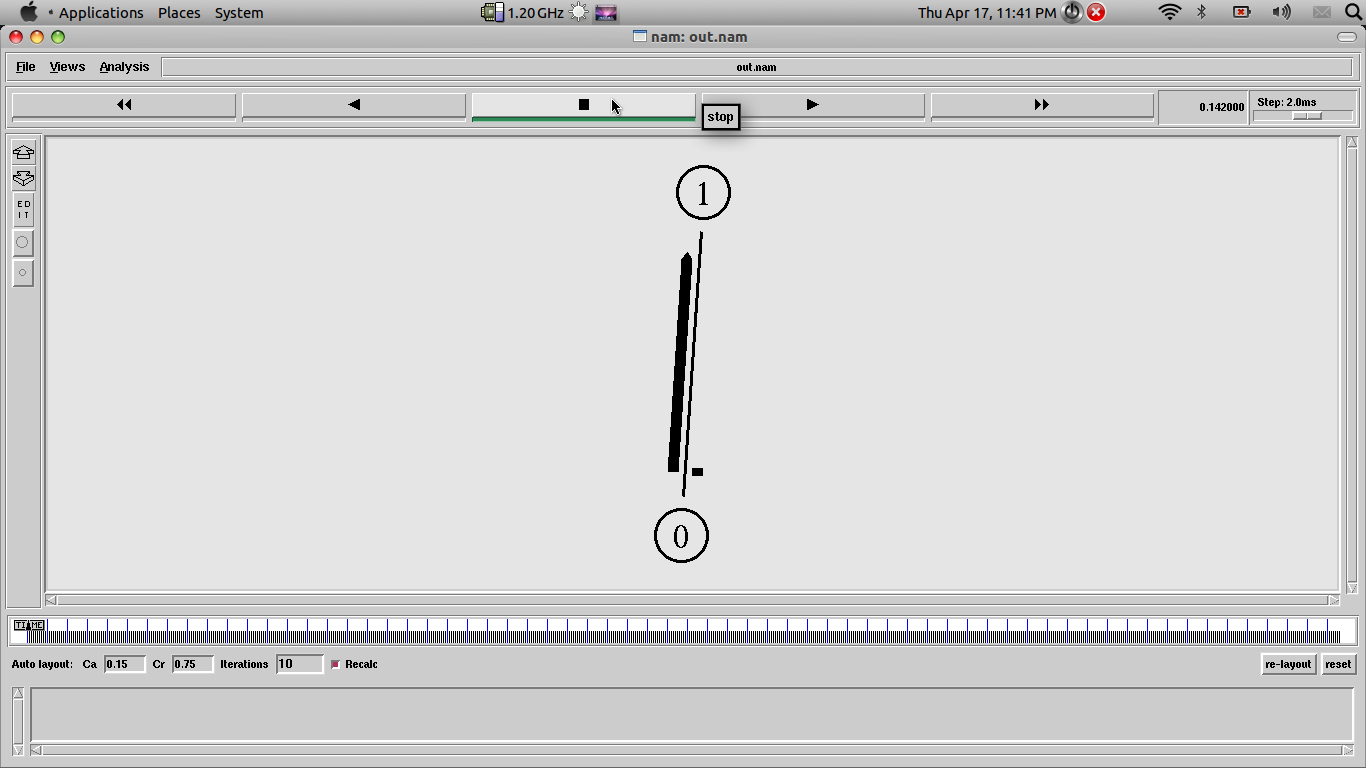
\includegraphics[bb=0 0 1232 493,scale=0.35]{working.png}
 % gaj1.png: 1232x493 pixel, 72dpi, 43.46x17.39 cm, bb=0 0 1232 493
\end{center}
\newpage






\section{Conclusion}
\begin{itemize}
 \item The topology has been made using tcl.
 \item The throughput has been calculated.
 \item The graph for inter arrival time vs sequence number has been plotted.
 \item We observe that the throughput is upper bounded by Minimum of link capacity and sending rate.
 \item In case of TCP, it automatically adapts its rate based on the congestion.
\end{itemize}
\newpage
\section{Implementation :}
\begin{itemize}
 \item The trace file generated has the format : \\
  \begin{center}
 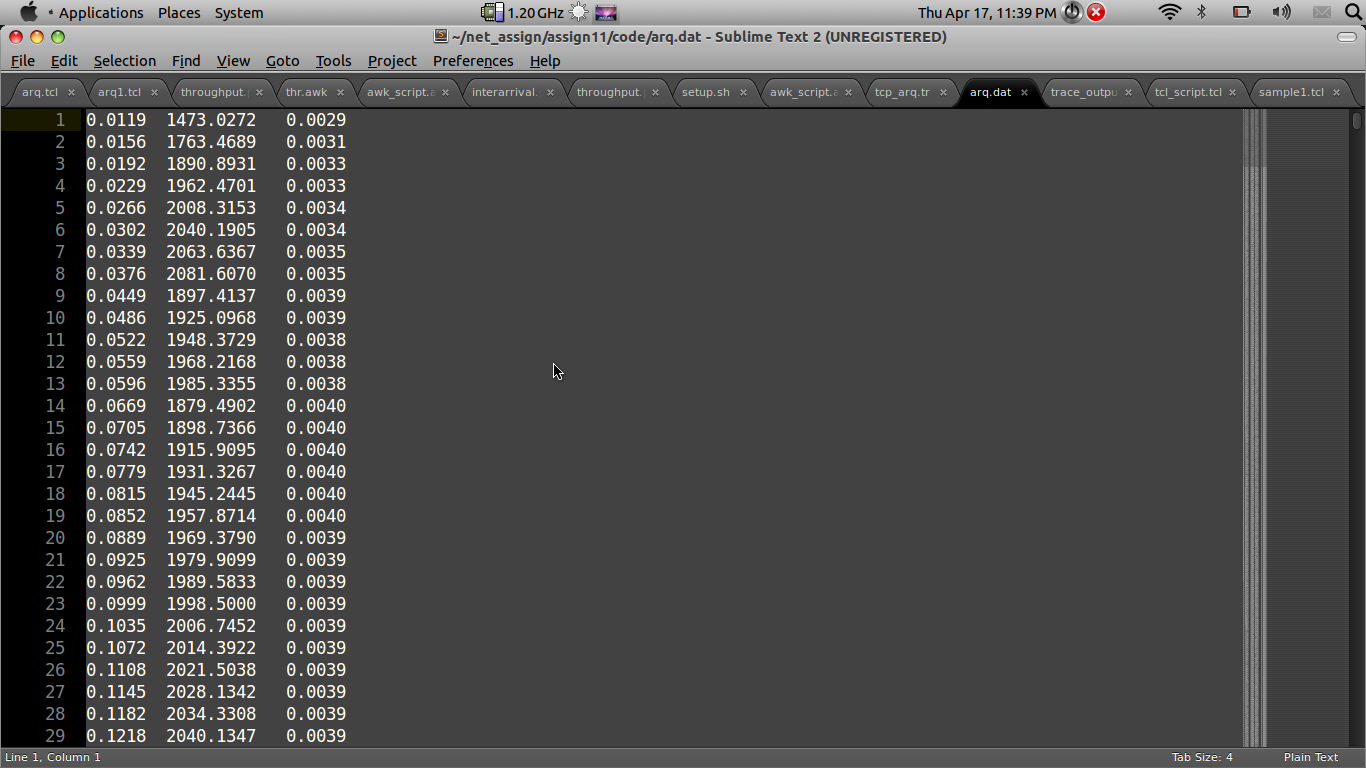
\includegraphics[bb=0 0 716 679,scale=0.35]{trace.png}
 % trace.png: 716x679 pixel, 72dpi, 25.26x23.95 cm, bb=0 0 716 679
\end{center}
\newpage
 \item Plot the graph  between retry limites and throwput.
 \begin{center}
 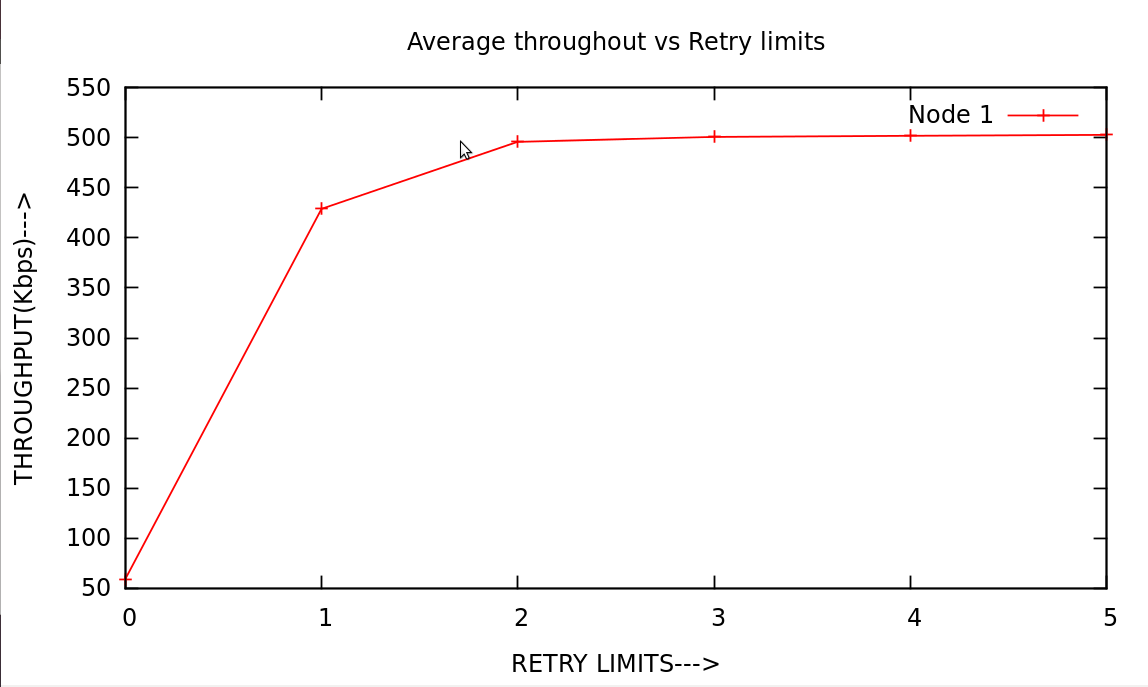
\includegraphics[bb=0 0 1148 687,scale=0.4]{retry.png}
 % gaj.png: 1148x687 pixel, 72dpi, 40.50x24.24 cm, bb=0 0 1148 687
\end{center}
\newpage
 \item Plot the graph  of Throughput.
 \begin{center}
 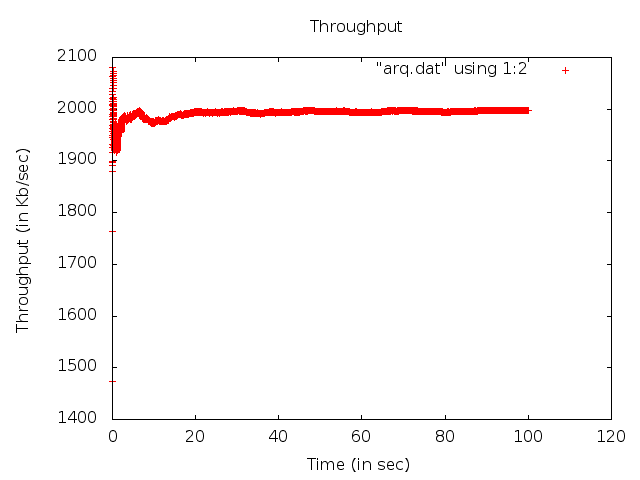
\includegraphics[bb=0 0 1148 687,scale=0.6]{throughput.png}
 % gaj.png: 1148x687 pixel, 72dpi, 40.50x24.24 cm, bb=0 0 1148 687
\end{center}
\newpage
 \item Plot the graph  of Interarrival Time.
 \begin{center}
 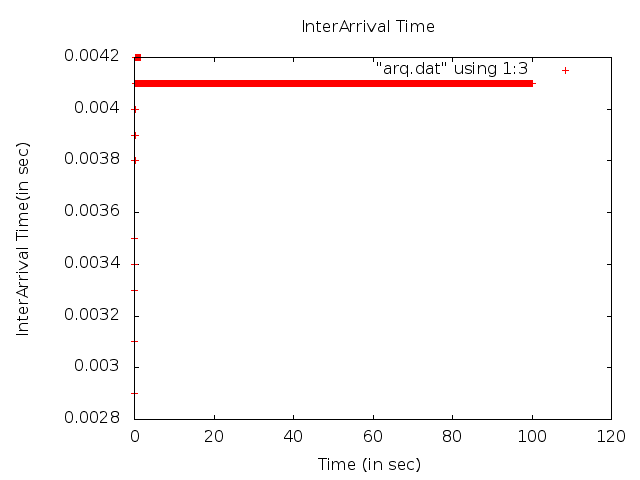
\includegraphics[bb=0 0 1148 687,scale=0.6]{interarrival.png}
 % gaj.png: 1148x687 pixel, 72dpi, 40.50x24.24 cm, bb=0 0 1148 687
\end{center}

 
 
\end{itemize}
\newpage

\end{document}
